\section{Discussion}
\label{discussion}

\Cref{results_section} presented results from generating the question dataset and running the framework to understand the role of parametric knowledge in question-answering.
This section attempts to explain these results, and discusses what they mean for our research question.

\subsection{Model architecture and memorised knowledge}
\label{model_architecture_parametric}

\Cref{framework_results} presents the results of running our framework on the provided questions on two different model architectures: Seq2Seq models and Decoder-only models.
\Cref{flan_cats_table,llama_cats_table} show these results split by category of question.

The results are clear: \textbf{Seq2Seq models tend to answer questions from their contextual knowledge rather than from their inherent knowledge more often than Decoder-only models}.
These results persist across different question categories and are consistent regardless of answer types and lengths

These results show that, in the framework of question-answering when using RAG to fetch contextual data from an index, Seq2Seq models will have fewer hallucinations that contradict this index than Decoder-only models.

We propose two hypotheses that could explain these differences.

\subsubsection{Advantages of the Encoder-Decoder Architecture}

As described in \cref{llm_architectures}, Seq2Seq models such as \texttt{Flan-T5} are encoder-decoder models that process the entire context of the query in the encoder component before passing it to the decoder, which could increase the weight given to the context itself.

We can test this hypothesis by finding the mean attention of the tokens corresponding to the context and to the rest of the query, and using the method discussed in \cref{attention_section}.

The results presented in \cref{attention_results} are consistent with this theory: Seq2Seq models allocate significantly more attention to the contextual tokens of the query compared to Decoder-only models.

\subsubsection{Different training data and fine-tuning}

It's possible that these result doesn't come from the model architecture, but the way the models are trained introduces some biases.

Additionally, the Flan models were trained on masked token generation and later fine-tuned on question-answering about passages \citep{flant5}.
This requires strong alignment between query and answer, which encourages the model to focus on the input context and makes it more likely to take the answer from the RAG-provided context.

Llama models were trained mainly on open-ended text generation, which relies more on parametric data.

It's possible that the deficiencies of knowledge grounding in Llama models might come simply to not being trained on related tasks.

\subsection{Model size and memorised knowledge}
\label{model_size_parametric}

\Cref{framework_results} also shows differences in how models of different sizes process information in queries with counterparametric context.

\subsubsection{Seq2Seq Models}

While the average results are very similar, which is likely due to the properties of Seq2Seq models discussed in \cref{model_architecture_parametric}, the models seem to be significantly different for queries of category \texttt{element}, \texttt{historical\_events}, and a few others.

Unfortunately, these results are due to failures on the models: for reasons not yet fully understood, \smallflan{} often produces nonsensical answers to questions requiring short responses, such as elements' names in the periodic table on historical dates.
This behaviour is different than \bigflan{}, which tends to provide correct answers in these cases.

When removing the categories with a significant amount of short answers and their nonsensical answers by the smaller model, the results of both Seq2Seq models seem similar.
Therefore, we can conjecture that \textbf{the size of a Seq2Seq model does not significantly affect its knowledge grounding}.

\subsubsection{Decoder-only Models}

\Cref{framework_results} shows a very different result for Decoder-only models.
Surprisingly, the smaller model \smallllama{} has \textit{better} knowledge grounding than the larger model \bigllama{}.

We already established that decoder-only models rely on parametric knowledge to a greater degree than Seq2Seq models.
Larger models have a vast internalised knowledge base accumulated from expensive training data, which can lead to increased confidence in their parametric knowledge.

It's possible that larger Decoder-only models are able to use their parametric knowledge to interpret the answer to the question in more ways that contradict the contextual knowledge.
The extra information encoder in its weights can produce more varied evidence against the contextual answer.

With this information, we can say that \textbf{the size of Decoder-only models \textit{does} affect its knowledge grounding, and when enhancing queries with RAG it might be preferable to use a smaller model}.

This is consistent with similar results found for other Decoder-only models, such as Pythia and GPT-2 \citep{factual_recall}.

\subsection{What are all of these Others?}

\Cref{parametric_vs_contextual} showed that a significant minority of responses to queries with counterfactual context are \Other{}: answers that aren't equal to either the parametric nor the contextual data.
The numbers of these entries, per model, are presented in \cref{others_list}.

\begin{table}[h]
	\centering
	\footnotesize
	\begin{tabular}{>{\bfseries}l | c c c c}
		\toprule
			& \ttfamily\scriptsize Flan-T5-XL & \ttfamily\scriptsize Flan-T5-XXL & \ttfamily\scriptsize \llamaparbox{} & \ttfamily\scriptsize \bigllamaparbox{} \\
		\midrule
			\Other{} & 260 & 192 & 312 & 387 \\
		\bottomrule
	\end{tabular}
	\caption{Amount of \Other{} entries, that is, results where the answer was not either the parametric or contextual answer.}
	\label{others_list}
\end{table}

By manually checking these results, we can understand the reason why the model chose these answers.

\begin{description}[style=nextline]
	\item[1. Different phrasing of a parametric answer]
		There are many answers where the parametric chooses a certain way to phrase some answer, while the contextual information biases it to give the parametric answer with a different context.
	\item[2. Plain incorrect answers]
		Sometimes, adding counterfactual context to the model just causes it to produce an incorrect answer that's different the answers given by both the model and the context.
	\item[3. Question misinterpretation due to the context]
		Some questions can be ambiguous or have a low probability of another answer.
		By adding a context with a counterfactual answer, the model can misinterpret the question and answer something different.
	\item[4. Negating the context]
		This is an interesting one: if the model has an answer in its parametric knowledge that contradicts the data on its context, then it interpret the context as part of the question and adds its negation as part of the answer.
	\item[5. Different phrasing of the context]
		Much less common than point 1, models sometimes give the same answer as the context but in the format of the parametric answer.
	\item[6. Correct answer, just different than the parametric answer]
		Some question have multiple correct answers, and adding counterfactual context can cause the model to give a different one.
	\item[7. Mixing elements of both parametric answer and context]
		Elements of the parametric answer are mixed with elements of the context in the model's answer.
		This produces an incorrect answer, but it's easy to understand where it came from.
		The cause of this is likely the greedy decoding used to find the answers, as explained in \cref{methodology_type_of_answer}.
\end{description}

Examples of each one of these types can be found in \cref{other_examples}.

Does the architecture and size of the model affect the distribution of each type of \Other{} answer?
\Cref{other_results_category} contains the amount of answers per architecture for each one of the models, and there does not seem to be a particular distribution.

\begin{table}[ht]
	\centering
	\footnotesize
	\begin{tabular}{>{\bfseries}r | r r r r}
		\toprule
			\bfseries Type & \ttfamily\scriptsize Flan-T5-XL & \ttfamily\scriptsize Flan-T5-XXL & \ttfamily\scriptsize \llamaparbox{} & \ttfamily\scriptsize \bigllamaparbox{} \\
		\midrule
			(\Parametric{}) & 248 & 242 & 745 & 1070 \\
			(\Contextual{}) & 4284 & 4304 & 3662 & 3303 \\
		\midrule
			1. & 0 & 0 & 116 & 234 \\
			2. & 6 & 3 & 50 & 15 \\
			3. & 0 & 0 & 13 & 8 \\
			4. & 0 & 0 & 20 & 61 \\
			5. & 241 & 170 & 33 & 38 \\
			6. & 7 & 16 & 63 & 23 \\
			7. & 6 & 3 & 17 & 8 \\
		\bottomrule
	\end{tabular}
	\caption{Different types of \Other{} answers per model (with amount of \Parametric{} and \Contextual{} added for comparison). The two most notable groups are \textbf{1.}, which contains parametric answers with different phrasing, and \textbf{5.}, which contains counterfactual answers with different phrasing.}
	\label{other_results_category}
\end{table}

Surprisingly, there is a large difference in the distribution of answers that don't come either from the model or from the given context.

In the case of Seq2Seq models, the vast majority of \Other{} answers are \Contextual{} answers which have a different format due to model mangling.
This is consistent with the previous result, where the vast majority of their answers came from the query's context.

The majority of \Other{} answers in Decoder-only models are the opposite: \Parametric{} answers that keep the format of the context.
However, the reasons are much more varied and this would be an interesting topic of discussion in future research.

Part of the reason for many of these answers, particularly on the Seq2Seq models, is due to the strict comparison function we use to define answer type.
This is an area that should be improved; \cref{other_problems} gives more information and various suggestions on how to compare results that might be relevant on future work.

\begin{table}[p]
	\centering
	\scriptsize
	\renewcommand{\arraystretch}{1.5}
	\begin{threeparttable}
		\begin{tabularx}{\textwidth}{>{\bfseries}c>{\ttfamily}X >{\ttfamily}p{75pt} >{\ttfamily}p{75pt} >{\ttfamily}p{75pt}}
			\toprule
			\bfseries Reason & \rmfamily\bfseries Question & \rmfamily\bfseries Parametric & \rmfamily\bfseries Counterfactual & \rmfamily\bfseries Contextual \\
			\midrule
			\multirow[t]{2}{*}{1.} & Who was the primary leader associated with The Reforms of Diocletian? & Diocletian Himself & Caracalla, a Roman Emperor & Diocletian, a Roman Emperor \\
			& In which city is Louvre Pyramid located? & Paris, France & the city of Valladolid, in the state of Yucatan, Mexico & the city of Paris, in the country of France \\
			\multirow[t]{1}{*}{2.} & In which period of the periodic table is Silver located? & 5 of the periodic table & 3 of the periodic table & 4 of the periodic table \\
			\multirow[t]{2}{*}{3.} & What was the duration of Queen Elizabeth II's Platinum Jubilee?	& 12 months & approximately 100 years & approximately 70 years \\
			& What is the nearest major body of water to Cusco? & Lake Titicaca & the North Sea & the Pacific Ocean \\
			\multirow[t]{2}{*}{4.} & What is the name of the main protagonist in One Flew Over the Cuckoo's Nest? & Randle McMurphy & Achilles & Not Achilles \\
			& What is Frida Kahlo primarily known for? & her self-portraits and her depiction of Mexican culture & his theories on communism and his critique of capitalism & her artwork and her life story, not for his theories on communism or critique of capitalism \\
			\multirow[t]{1}{*}{5.} & How many pages are in One Flew Over the Cuckoo's Nest? & 320 pages	& 480 pages in a standard edition & 480 pages \\
			\multirow[t]{3}{*}{6.} & Who is credited with the discovery of Conservation of Energy? & Julius Robert Mayer & Alfred Wegener & James Joule\tnote{1} \\
			& What is the name of the main protagonist in The Great Gatsby? & Nick Carraway	& Liesel Meminger & Jay Gatsby\tnote{2} \\
			& What educational institution did Srinivasa Ramanujan attend? & The University of Madras & The University of Vienna & the University of Cambridge\tnote{3} \\
			\multirow[t]{2}{*}{7.} & What is the date of death of Vladimir Lenin? & January 21, 1924 & March 28, 1941 & March 21, 1924 \\
				& What's the main nationality of Mozart? & Austria & English-Born American & American-born English-born Austrian \\
			\bottomrule
		\end{tabularx}
		\begin{tablenotes}
\item[1] Discovery of the conservation of energy is credited to both Julius Robert Mayer and James Joule.
\item[2] Nick Carraway and Jay Gatsby are co-protagonists in The Great Gatsby.
\item[3] Srinivasa Ramanujan attended both the University of Madras and the University of Cambridge.
		\end{tablenotes}
	\end{threeparttable}
	\caption{Examples of different types of \Other{} answers when running the \texttt{Meta-Llama-3.1-8B-Instruct} model. Other models have similar reasons for these kinds of answers.}
	\label{other_examples}
\end{table}

\subsection{Differences in distribution of perplexity scores}

The distribution of perplexity scores, shown in \cref{results_perplexity_score}, shows a significant difference in the perplexity scores between \Parametric{} and \Contextual{} answers for all four models.
This is even more marked on Seq2Seq models, where for both models the 90\% percentile of the \Contextual{} answer is lower than the 10\% percentile of the \Parametric{}.

In fact, this confirms our conjecture that \textbf{models tend to be surprised when finding an answer that contradicts the context of the query}.
This conjecture seems to be true regardless of model size or question type (see \cref{flan_catboxes,llama_catboxes}).

The cause for the difference in the perplexity values for different architectures is likely the same as discussed in \cref{model_architecture_parametric} on why the \texttt{Flan-T5} models generally have better performance on these tasks than \texttt{Llama} models.
\begin{description}
	\item[Model Architecture] By processing the entire input in one go, the Seq2Seq encoding step processes information in the context in the encoding step first before starting decoding. In Decoder-only models, the shift from going from contextual to parametric knowledge is less abrupt, resulting in a less pronounced change in perplexity.
	\item[Training Data] \texttt{Flan-T5} models are trained in data where getting information from the query itself is more relevant.
		In a sense, they are biased to being more surprised when producing a parametric answer.
\end{description}

\subsubsection{Can we use the perplexity to predict the source of an answer?}

Seeing the current results, it's tempting to attempt to create a model that can predict, with perplexity information alone and without making any extra query, whether the answer in a query with added context came from the \Parametric{} knowledge of the context or from the \Contextual{} information in the query.

This can be useful in practice: if a RAG-enhanced model finds an answer with high perplexity, it can attempt to re-run the RAG indexing to find a more relevant answer and possible prevent a hallucination.

The results in \cref{perplexity_flan_table,perplexity_llama_table} seem consistent with \cref{roc_auc} in that such predictor would work better in Seq2Seq models, particularly on \bigflan{}: by re-running the RAG indexer on answers with perplexity over 1.5, we can prevent hallucinations on 90\% of the answers that came from parametric knowledge while keeping 80\% of the total.

\begin{figure}[hb]
	\centering
	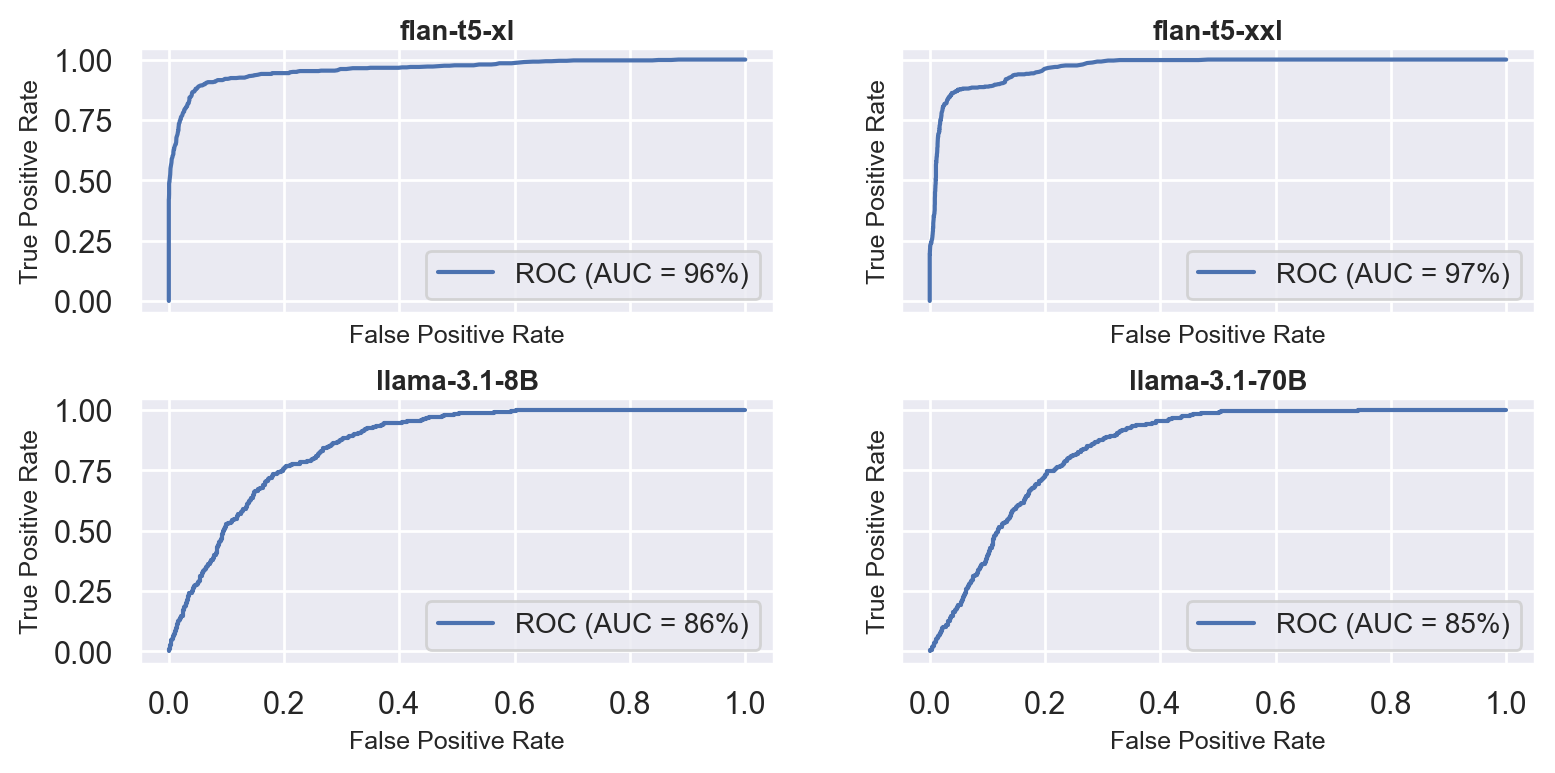
\includegraphics[width=.85\textwidth]{roc_auc.png}
	\caption{ROC curve of the four tested models to find out whether an answer came from the \Parametric{} knowledge of a model using the perplexity of the answer.}
	\label{roc_auc}
\end{figure}
